%!TEX program = xelatex
\documentclass[10pt,aspectratio=169]{ctexbeamer}
% !TeX root = main.tex
% 继承 ustcbeamer 的科大蓝、校徽和 Beamer 字体机制；正文采用白底讲义式母版。
\usepackage[bluetheme]{ustcbeamer}
\usepackage{array,booktabs,tabularx}
\usetikzlibrary{calc,arrows.meta}
\IfFontExistsTF{Microsoft YaHei}{\setCJKsansfont{Microsoft YaHei}}{}
\IfFontExistsTF{Arial}{\setsansfont{Arial}}{}
\definecolor{navy}{HTML}{0C315B}
\definecolor{ink}{HTML}{19334E}
\definecolor{slate}{HTML}{52697D}
\definecolor{hair}{HTML}{CBD7E2}
\definecolor{teal}{HTML}{007D78}
\definecolor{rust}{HTML}{AA462B}
\definecolor{wash}{HTML}{EBF2F8}
\definecolor{nightblue}{HTML}{072A52}
\setbeamercolor{normal text}{fg=ink,bg=white}
\setbeamercolor{frametitle}{fg=themecolor,bg=white}
\setbeamercolor{insight}{fg=ink,bg=wash}
\setbeamertemplate{navigation symbols}{}
\setbeamersize{text margin left=.74cm,text margin right=.74cm}
\setbeamertemplate{headline}{\hbox{\color{themecolor}\rule{\paperwidth}{1.35pt}}}
\newcommand{\chaptermarkno}{00}
\newcommand{\parttitle}[2]{\renewcommand{\chaptermarkno}{#1}\section{#2}}
\newcommand{\reportSource}{}
\newcommand{\source}[1]{\renewcommand{\reportSource}{#1}}
\setbeamertemplate{frametitle}{%
  \vskip.17cm
  \hbox to \textwidth{%
    \vbox{\hbox{\fontsize{7.3}{9}\selectfont\bfseries\color{teal}\chaptermarkno\hspace{.13cm}/\hspace{.13cm}\insertsectionhead}%
          \vskip.06cm
          \hbox{\fontsize{15.4}{18}\selectfont\bfseries\color{themecolor}\insertframetitle}}%
    \hfil\raise.03cm\hbox{
\includegraphics[width=.71cm]{figures/ustc_logo.pdf}}}%
  \vskip.13cm{\color{hair}\hrule height .45pt}\vskip.04cm}
\setbeamertemplate{footline}{%
  \leavevmode\hbox{\hspace{.74cm}\begin{minipage}{14.52cm}
  {\color{hair}\hrule height .4pt}\vspace{.075cm}
  {\fontsize{6.1}{7.4}\selectfont\color{slate}中国科学技术大学\hfill
    \reportSource\hfill\textbf{\insertframenumber}\,/\,\inserttotalframenumber\par}
  \end{minipage}}\vskip.12cm}
\setlength{\tabcolsep}{4pt}
\renewcommand{\arraystretch}{1.25}
\newcolumntype{Y}{>{\raggedright\arraybackslash}X}
\newcommand{\key}[1]{\textcolor{themecolor}{\textbf{#1}}}
\newcommand{\warm}[1]{\textcolor{rust}{\textbf{#1}}}
\newcommand{\cool}[1]{\textcolor{teal}{\textbf{#1}}}
\newcommand{\minor}[1]{\par\smallskip{\fontsize{8.1}{10.6}\selectfont\color{slate}#1\par}}
\newcommand{\subhead}[1]{\par{\fontsize{11.2}{14}\selectfont\color{themecolor}\bfseries #1\par}\vspace{.10cm}}
\newcommand{\tagline}[1]{{\fontsize{8.1}{10}\selectfont\bfseries\color{teal}#1\par}\vspace{.10cm}}
\newcommand{\entry}[2]{\subhead{#1}#2\par}
\newcommand{\gap}{\par\vspace{.29cm}}
\newcommand{\insight}[2]{\par\vspace{.16cm}\begin{beamercolorbox}[wd=\linewidth,sep=.18cm]{insight}%
  \small\key{#1}\hspace{.17cm}#2\end{beamercolorbox}}
\newcommand{\bignum}[1]{{\fontsize{22}{25}\selectfont\bfseries\color{themecolor}#1\par}}
\newcommand{\thd}[1]{\textcolor{navy}{\bfseries #1}}
\newcommand{\refurl}[2]{\href{#1}{\textcolor{themecolor}{#2}}}
\newcommand{\chart}[1]{\includegraphics[width=\linewidth]{figures/report/#1.pdf}}
\setbeamertemplate{itemize items}{\small\color{teal}\textbullet}
\hypersetup{unicode=true,colorlinks=true,urlcolor=themecolor,linkcolor=themecolor}

% 项目组确认的分工见 main.tex；封面与分工页共用以下姓名。
\newcommand{\memberA}{高宇娇}
\newcommand{\memberB}{尹弘毅}
\newcommand{\memberC}{何梓慕}
\newcommand{\memberD}{刘金时}
\newcommand{\presenter}{\memberD}

\newcommand{\campusrows}{%
北城高铁站 & 21:36 & 22:00 \\
新桥2号航站楼 & 21:45 & 22:15 \\
合肥火车站 & 22:15 & 22:48 \\
合肥南站 & 22:22 & 23:35 \\
中国科大东区 & 22:28 & 22:39 \\
图书馆 & 22:39 & 23:52 \\%
}

\title{合肥轨道交通的换乘可达性}
\subtitle{换乘中断、夜间加班与分时客流预测}
\author{复杂系统分析课程项目组}
\institute{中国科学技术大学}
\date{线网快照：2026-11-23}

\begin{document}

% 01 — 封面。右侧纹样由本项目边表与示意坐标生成。
\begin{frame}[plain]
\begin{tikzpicture}[remember picture,overlay,shift={(current page.south west)},inner sep=0pt]
  \shade[left color=nightblue,right color=navy] (0,0) rectangle (16,9);
  \node[opacity=.70] at (13.25,4.05) {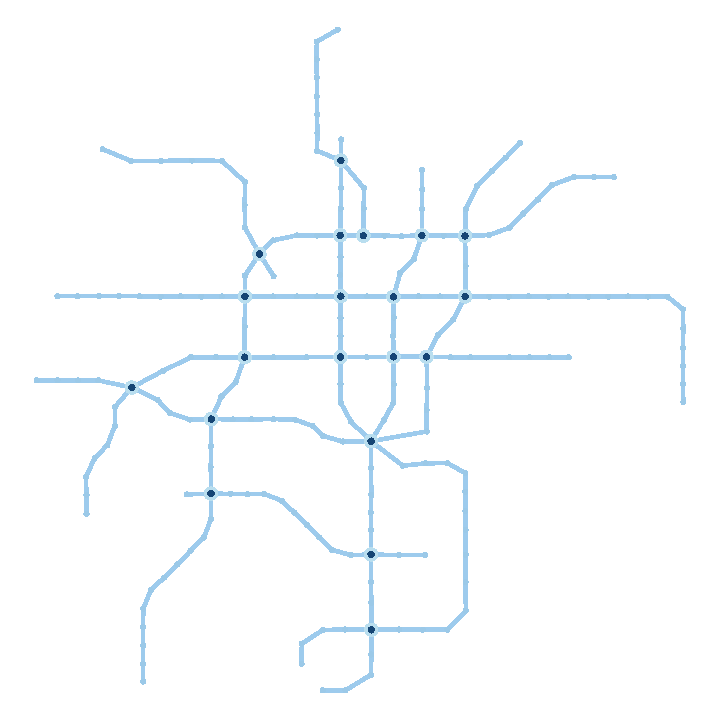
\includegraphics[width=7.05cm]{figures/report/cover-network.pdf}};
  \fill[teal!55!cyan] (.84,7.72) rectangle (1.04,7.80);
  \node[anchor=west,text=white,font=\small\bfseries] at (1.20,7.76) {复杂系统分析\quad /\quad 期末项目汇报};
  \fill[white] (14.94,7.96) circle (.41);
  \node at (14.94,7.96) {
\includegraphics[width=.79cm]{figures/ustc_logo.pdf}};
  \node[anchor=west,text=white,font=\fontsize{22.5}{27}\selectfont\bfseries] at (.84,5.22) {\inserttitle};
  \node[anchor=west,text=white!88!nightblue,font=\fontsize{12}{15}\selectfont] at (.88,4.28) {\insertsubtitle};
  \draw[white!48!nightblue,line width=.5pt] (.88,3.68)--(8.75,3.68);
  \node[anchor=west,text=white,font=\small] at (.9,2.55) {中国科学技术大学\quad ·\quad 汇报：\presenter};
  \node[anchor=west,text=white!73!nightblue,font=\footnotesize] at (.9,1.28) {1--8 号线及 S1\qquad 线网与时刻快照\enspace 2026.11.23};
\end{tikzpicture}
\note{从机场搭上末班车，能到西站却未必能换上下一班。同样是关键站，有的决定有没有路，有的决定赶不赶得上；再加入分时客流后，还能问哪些站在不同时段值得优先关注。}
\end{frame}

\parttitle{00}{研究路线}
\source{复杂系统分析 · 期末项目}
\begin{frame}{目录}
\centering
\begin{minipage}{.72\linewidth}
\tagline{汇报结构}
{\large\renewcommand{\arraystretch}{1.48}\begin{tabular}{@{}ll@{}}
\key{01} & 研究范围、数据与网络建模\\
\key{02} & 实验一：站内换乘中断\\
\key{03} & 实验二：末班衔接与加开晚班\\
\key{04} & 实验三：分时客流与关键站预测\\
\key{05} & 结果复核、分工与答疑
\end{tabular}}
\end{minipage}\par
\note{三个实验回答三个问题：换乘口用不了，还有路吗？末班之后加一趟，能接通哪些行程？同一张网里，早晚出行分布不一样，关键站名次会不会变？最后给出数据和复核路径。}
\end{frame}

\parttitle{01}{研究范围、数据与建模}
\source{站序与换乘：高德合肥地铁；示意坐标：MetroMan}
\begin{frame}{同一张合肥地铁网，三个问题}
\begin{columns}[c,onlytextwidth]
\column{.54\textwidth}
\chart{network}
\minor{大圆表示换乘站。}
\column{.43\textwidth}
\entry{实验一：如果不能换线，还有路吗？}{合肥南站有三线交会，S1 却只能在合肥西站换线。若一座站不能换乘，哪些起终点站对（OD）会失联，哪些要绕行？}
\gap
\entry{实验二：有路，还赶得上车吗？}{用逐班时刻检验：在哪条线加车，能让更多起终点重新接得上？}
\gap
\entry{实验三：早晚关键站一样吗？}{保留全站点，用公开客流与地理数据估算分时出行，再给各站重新排名。}
\end{columns}
\note{图上的大圆是换乘站。机场方向只能经西站换线，南站却连接三条线。先用换乘中断找到替代路径，再用末班时刻验证这些路夜间能否接通。最后，白天的线路并没有换位置，但乘客的起点和去向在变，看看站点名次是否跟着变。}
\end{frame}

\source{输入：metro\_edges.csv、night\_trips.csv、night\_last\_departures.csv}
\begin{frame}{数据来源与处理}
\tagline{合肥 1--8 号线及 S1\qquad 运营日：2026 年 11 月 23 日（周一）}
{\small\renewcommand{\arraystretch}{1.55}
\begin{tabularx}{\linewidth}{@{}Y p{4.0cm}@{}}
\toprule\thd{收集了哪些数据} & \thd{数据来源}\\\midrule
\key{线网结构}：各线站名、站序，以及哪些线路能在同一站换乘。 & \refurl{https://www.amap.com/ssr/subway/hefei-3401}{高德地图 · 合肥地铁线网}\\
\key{日间时刻}：每条线两个方向各取一趟中午列车的逐站时刻。 & \refurl{https://www.metroman.cn/en/planner/hefei}{MetroMan · 合肥路线规划}\\
\key{夜间班次}：449 趟列车的方向、运行区段和逐站时刻。 & \refurl{https://www.metroman.cn/en/planner/hefei}{MetroMan · 合肥路线规划}\\
\key{逐站末班}：按车站、线路和方向记录的 432 条末班发车时刻。 & \refurl{https://www.metroman.cn/en/cities/hefei/stations/hefei-xizhan-hefeixi-railway-station}{MetroMan · 车站时刻表}\\\bottomrule
\end{tabularx}}
\minor{时刻取自规划平台，并非实测。线网图的示意坐标取自 MetroMan，仅用于绘图。}
\note{高德线网图用来核对站序和换乘关系。时间数据分开收：中午取同一趟车的相邻站时刻，用于估计运行时间；夜间保留整趟车的逐站时刻，才能判断能否接上下一班。最后用站页的四百三十二条末班记录逐项核对。两种时刻页面都来自 MetroMan，不是两个独立来源。}
\end{frame}

\source{构图：src/build\_network.py\qquad 基线：results/metro.graphml}
\begin{frame}{建网方法}
\begin{columns}[c,onlytextwidth]
\column{.55\textwidth}
\tagline{局部示意\quad /\quad 合肥南站}
\begin{tikzpicture}[x=1cm,y=1cm,inner sep=1pt,font=\footnotesize]
  \draw[slate,dashed,thick] (3.70,3.13)--(3.70,.53);
  \draw[slate,dashed,thick] (3.70,3.13) .. controls (5.50,2.88) and (5.50,.78) .. (3.70,.53);
  \foreach \y/\linecol/\id/\prev/\nextstop in {3.13/rust/1/南站南广场/望湖城,1.83/themecolor/4/望湖城南/淝南,.53/teal/5/望湖城西/盛大}{
    \draw[\linecol,line width=1.4pt] (1.14,\y)--(6.93,\y);
    \node[anchor=east,text=\linecol,font=\footnotesize\bfseries] at (.94,\y) {\id 号线};
    \foreach \x in {1.60,6.43}{\draw[draw=\linecol,fill=white,line width=.9pt] (\x,\y) circle (.065);}
    \draw[draw=\linecol,fill=white,line width=1.3pt] (3.70,\y) circle (.115);
    \node[above=2pt] at (1.60,\y) {\prev};\node[above=2pt] at (6.43,\y) {\nextstop};
  }
  \node[above=3pt,text=navy,font=\small\bfseries] at (3.70,3.13) {合肥南站};
\end{tikzpicture}
\minor{实线：同线运行。虚线：同站换线，基准每次 5 分钟。}
\column{.41\textwidth}
\entry{节点：换乘站按线路拆开}{普通站是一个节点；换乘站每条线各设一个。图中合肥南站对应三个节点，全网 204 座车站展开为 225 个节点。}
\gap
\entry{边：构成无向加权图}{216 条实线连接同线相邻站，权重取双向运行时间的均值；22 条虚线连接同站不同线路，每条计 5 分钟。两类边都可双向通行。}
\end{columns}
\insight{消融单位}{关南站换乘，就同时去掉三条虚线。列车仍停靠，乘客仍可从本站任一线路出发或到达。}
\note{顺着图上的任一条实线，乘客可以不换车经过合肥南站；从一个南站节点走到另一个，才需要经过虚线，付出五分钟的换乘代价。实验一只删虚线，不关站、不停列车。后面比较介数时才把同站节点合并，出行的起点和终点也始终按物理站计数。}
\end{frame}

\parttitle{02}{实验一 · 站内换乘中断}
\source{协议：固定线网、等权 OD、相同关闭预算；不模拟列车停运}
\begin{frame}{实验设计}
\begin{columns}[T,onlytextwidth]
\column{.48\textwidth}
\tagline{基线与评价}
\entry{20,706 对无序 OD}{用 Dijkstra 算最短分钟；起终点可任选本车站的线路副本。基线全部可达，均值为 42.00 分钟。}
\gap
\entry{两类损失}{失联单列一组；仍可达时，比较中断前后的最短时间。不能给失联任意填一个惩罚分钟数。}
\column{.48\textwidth}
\tagline{干预与对照}
\entry{单站：逐个试 20 次}{先按失联 OD 数、再按仍可达组平均额外分钟降序排出损失名次，与原始介数对照。}
\gap
\entry{多站：每次再关一座}{按初始介数、单站损失、随机排列分别从 0 关到 20 座；顺序预先固定，不边关边重排。}
\end{columns}
\note{这里的损失名次是一条事先声明的优先规则：完全走不通优先于还可绕行；有相同失联对数，再比较所有仍可达行程的平均额外时间。随机对照排除单纯因为多关了几座站而更差的解释。每条序列内，前面关掉的站不会恢复。}
\end{frame}

\source{原图：换乘消融实验 §2；results/transfer\_ablation/single\_station.png}
\begin{frame}{单站：失联、变慢是不同的影响}
\begin{columns}[c,onlytextwidth]
\column{.705\textwidth}
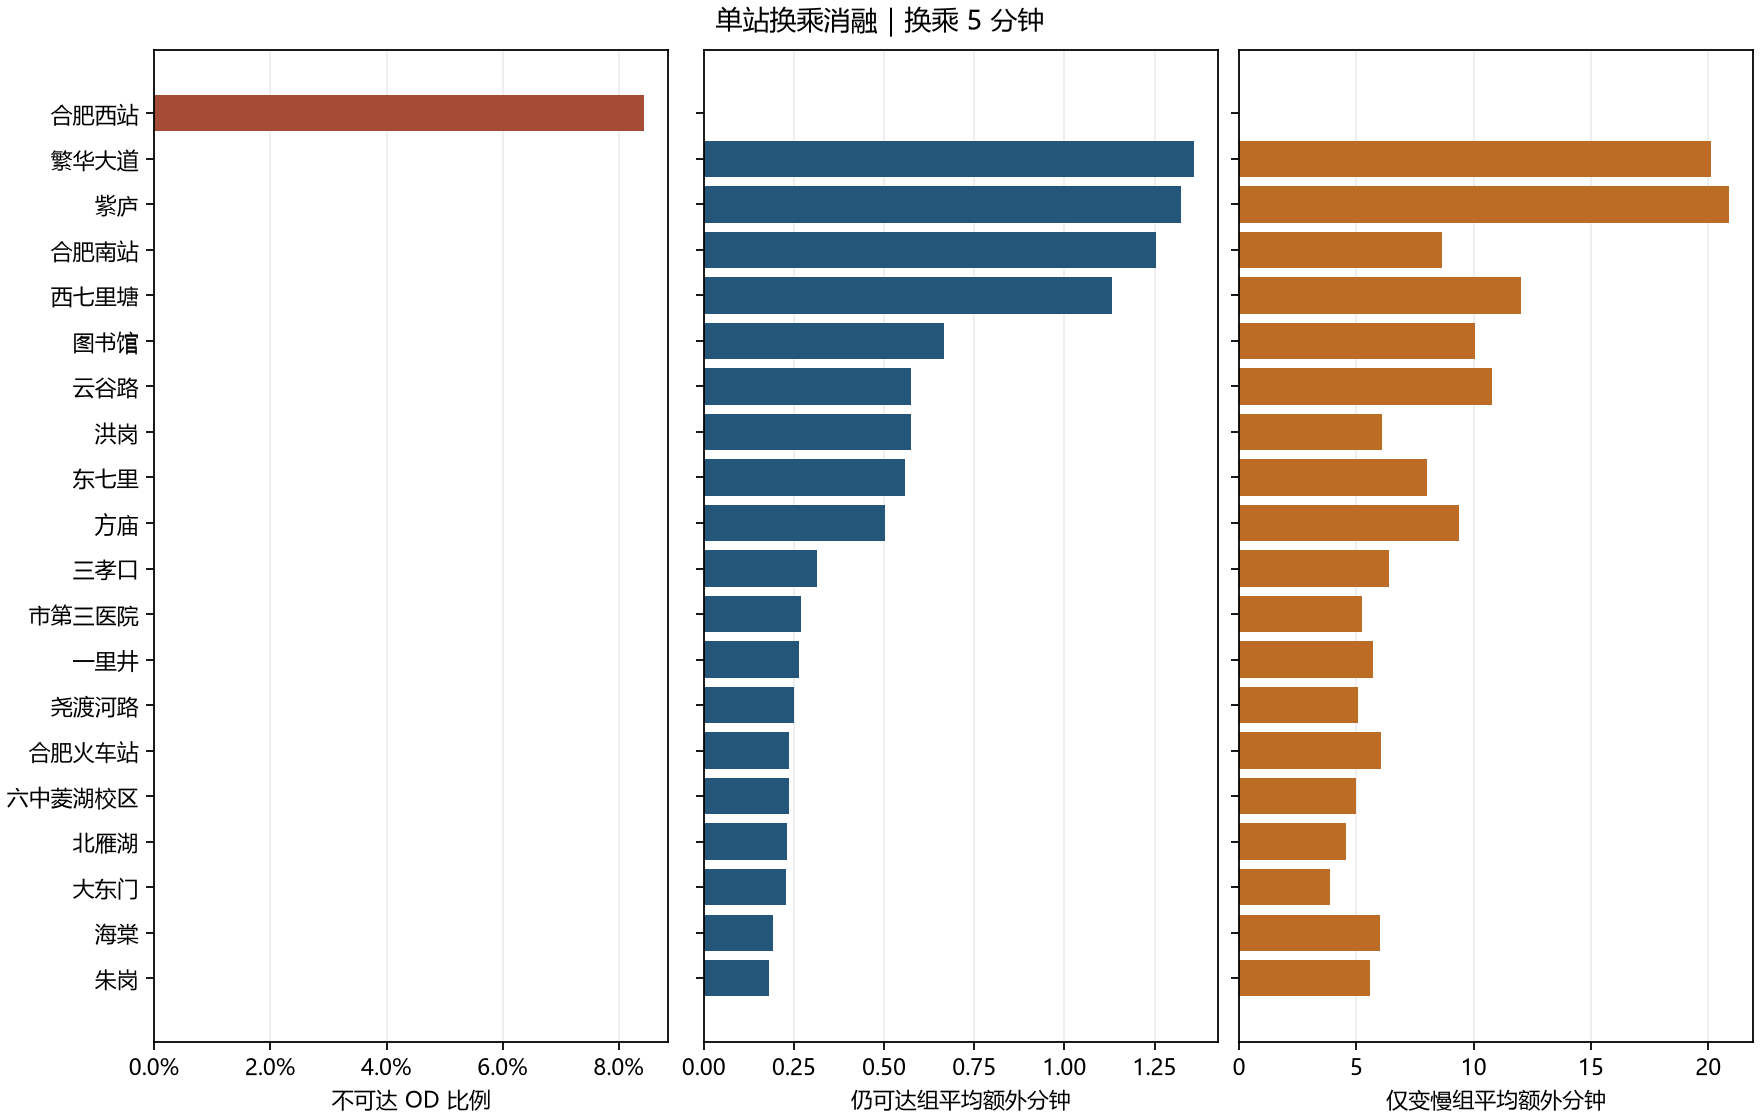
\includegraphics[width=\linewidth,height=6.48cm,keepaspectratio]{../../results/transfer_ablation/single_station.png}
\column{.26\textwidth}
\tagline{每行关闭一站的换乘}
\entry{左：走不通}{失联对数占全部 20,706 对的比例。}
\gap
\entry{中：还能到}{平均多花几分钟，包含没有变慢的行程。}
\gap
\entry{右：确实变慢}{只在耗时增加的行程中取平均。}
\end{columns}
\note{横向读同一行。只有合肥西站在左图有柱；它右图为空，不是损失为零，而是仍可达的站点对都没变慢。繁华大道和紫庐则相反，没有站点对失联，真正要绕路的那批行程却平均多花二十多分钟。三个横轴的单位和分母不同，不能直接比较柱长。}
\end{frame}

\source{单站结果：results/transfer\_ablation/single\_station.csv；路径复核：分钟图}
\begin{frame}{行程失联与绕远}
\tagline{同一基线\quad /\quad 四个代表站；全表 20 站}
{\small\begin{tabular*}{\linewidth}{@{\extracolsep{\fill}}lrrrr@{}}
\toprule\thd{不能换乘的站} & \thd{去掉换乘边} & \thd{失联 OD} & \thd{变慢 OD} & \thd{仅变慢组平均多花（分）}\\\midrule
\key{合肥西站} & 1 & \warm{1,746} & 0 & ---\\
\key{合肥南站} & 3 & 0 & \key{3,003} & 8.65\\
繁华大道 & 1 & 0 & 1,399 & 20.10\\
紫庐 & 1 & 0 & 1,313 & 20.88\\\bottomrule
\end{tabular*}}
\gap
\begin{columns}[T,onlytextwidth]
\column{.30\textwidth}\subhead{西站：唯一的换乘口}
\small 西站一处中断，S1 独有的 9 站与其余非 S1 的 194 站失联；S1 线内仍可乘坐。
\column{.30\textwidth}\subhead{南站：变慢的行程最多}
\small 3,003 对仍能到，但要绕行。义兴至南屏路从 19 分钟增至 50 分钟。
\column{.34\textwidth}\subhead{繁华大道、紫庐：短途绕远}
\small 两站各自中断都不致失联，但变慢组平均多花约 20 分钟。紫庐中断后，塘西河公园至滨湖医院从 10 分钟增至 74.5 分钟。
\end{columns}
\note{这里统计的是站点对，不是线路数或乘客数。二十个单站情景中，只有合肥西站不能换乘时出现失联。合肥南站影响的行程最多，而繁华大道和紫庐的特点是少数本来很短的路径要绕很远。例如，繁华大道不能换乘时，大学城北至翡翠公园从八点五分钟变为七十七分钟。两个算例都按同一张五分钟换乘图重算，不是全站平均。}
\end{frame}

\source{比较对象：20 座换乘站；两轴均为名次，1 为最高}
\begin{frame}{介数与换乘损失}
\begin{columns}[c,onlytextwidth]
\column{.58\textwidth}\chart{rank-comparison}
\minor{每点一站；虚线表示两种名次完全相同。}
\column{.38\textwidth}
\tagline{Spearman 秩相关}
\bignum{$\rho=0.346$}
\smallskip 两份前五名名单，只有\key{合肥南站}重合。\par
\gap
\entry{看偏离对角线的站}{洪岗：介数第 1，损失第 8。\\合肥西站：介数第 13，损失第 1。}
\end{columns}
\insight{解释}{介数统计正常网络里哪些站常被经过；消融实验问的是失去换乘后，有没有可用的替代路径。}
\note{请看虚线两侧。介数高说明很多最短路途经洪岗，不意味着它一旦不能换乘，所有这些人都没有选择。反过来，西站未必出现在最多最短路上，却是机场方向跨线的唯一接口。这个相关系数是该线网的描述统计，不是事故概率，也不是显著性检验。}
\end{frame}

\source{multi\_station.csv；阴影为随机序列的 2.5\%--97.5\% 经验分位区间，不是置信区间}
\begin{frame}{不同换乘中断顺序的对比}
\chart{closure-curves}
\begin{columns}[T,onlytextwidth]
\column{.48\textwidth}\small\key{看前 3 站。}介数顺序失联 0，随机平均 1.73\%；按损失先关西站、繁华大道、紫庐，7 号线两个换乘口也同时消失。
\column{.48\textwidth}\small\key{看全过程。}用全体 OD 的最短时间倒数均值衡量效率，失联贡献 0，再除以正常效率；即使尚未失联，绕远也会拉低效率。
\end{columns}
\note{请先读左图同一个横坐标，而不是比较不同步的端点。繁华大道和紫庐单独关都不失联，但一起关就让七号线失去全部换乘口，组合后果不能相加。右图保留了仍可达却变慢的代价。灰带是不同随机顺序本身的离散程度，不是对真实事故作出的概率预测。}
\end{frame}

\source{固定样本复核：summary.json → fixed\_cohort；介数顺序第 12 站为方庙}
\begin{frame}{平均绕行时间}
\begin{columns}[c,onlytextwidth]
\column{.58\textwidth}
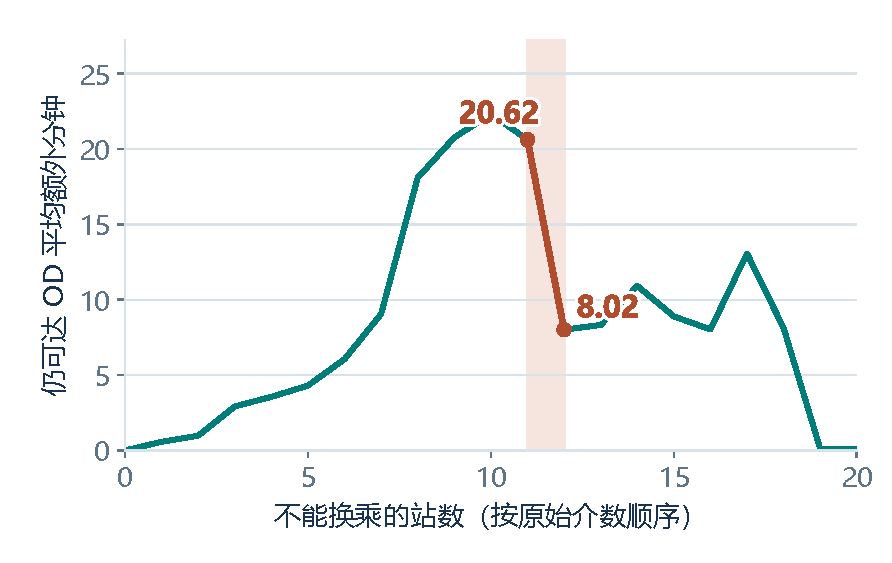
\includegraphics[width=\linewidth,height=4.85cm,keepaspectratio]{figures/report/detour.pdf}
\minor{每一步都只统计当时仍可达的 OD，包含未变慢的行程。}
\column{.38\textwidth}
\entry{第 12 站：方庙}{仍可达 OD 从 18,426 对减至 12,032 对。退出的 6,394 对原先平均多绕 \warm{44.58 分钟}，失联后不再计入均值。}
\gap
\entry{固定同一批 OD 再看}{只比较两步都可达的 12,032 对，平均额外时间从 \key{7.88 分}增至 \key{8.02 分}，并没有变快。}
\end{columns}
\insight{为什么曲线下降？}{从 20.62 分降到 8.02 分，是因为原先绕得远的行程失联了，而不是因为出现了更短的路。}
\note{注意图里的红线。按介数顺序多关一站，最短路不可能因为少了一条边而变短。左图每次都重新挑出仍可达的行程，所以两点平均的不是同一批。把相同的站对留下再比较，绕行反而略有增加。这也是前面要单独报告不可达比例的原因。}
\end{frame}

\source{summary.json → settings；AUC 是相对效率对关闭比例的梯形积分}
\begin{frame}{把换乘设为 3、5、7 分钟的结论}
\tagline{只改换乘权重；各参数下分别重算正常效率，多站实验沿用基准站序}
{\small\begin{tabular*}{\linewidth}{@{\extracolsep{\fill}}lcrrr@{}}
\toprule\thd{换乘成本} & \thd{单站损失第一} & \thd{随机平均 AUC} & \thd{介数顺序 AUC} & \thd{损失顺序 AUC}\\\midrule
3 分钟 & 合肥西站 & 0.7491 & 0.7143 & 0.7129\\
\key{5 分钟} & \key{合肥西站} & \key{0.7603} & \key{0.7277} & \key{0.7252}\\
7 分钟 & 合肥西站 & 0.7691 & 0.7381 & 0.7350\\\bottomrule
\end{tabular*}}
\gap
\subhead{AUC 怎么算？}
\small 关闭 $k$ 座站的换乘后，把所有 OD 的最短时间倒数取平均（失联计 0），再除以正常效率，记为 $R_k$。横轴为关闭比例 $k/20$，每步宽 $1/20$，用梯形面积求和：
\[
  \mathrm{AUC}=\sum_{k=1}^{20}\frac{R_{k-1}+R_k}{2}\cdot\frac{1}{20}.
\]
\minor{同一行内，面积越小，全程保留的效率越少。随机列是 100 条随机顺序各自 AUC 的平均。}
\note{每相邻两个关闭比例之间画一个梯形。梯形的高取两端相对效率的平均，宽是二十分之一；二十段相加就是表里的面积。三种换乘成本分别重算各自的正常效率，所以在同一行内比较。西站在三种成本下都排第一；两套固定顺序的面积都低于随机平均，彼此差距不大。}
\end{frame}

\parttitle{03}{实验二 · 末班车衔接}
\source{逐班时刻：449 趟；算法：src/night\_ablation.py → latest\_boarding}
\begin{frame}{实验二：设计与计算方法}
\begin{columns}[T,onlytextwidth]
\column{.48\textwidth}
\tagline{实验设计}
\entry{什么会消失？}{时钟向前，已从本站开走的班次不能再上车；已在车上的人仍可续乘。按方向分别统计 $204\times203$ 对 OD。}
\gap
\entry{和谁比较？}{以原时刻表为基线，先逐线加开，再比较三条线一起加开。原有班次全部保留。}
\column{.48\textwidth}
\tagline{计算方法}
\entry{从晚到早扫描各站的发车事件}{上车后可到下一站，也可原车往下坐；若下一趟的发车不早于“到站时刻＋缓冲”，还能接上那趟车。跨线留 5 分钟，同线换车留 1 分钟。}
\gap
\entry{记录最晚首程 $L_{od}$}{对起点 $o$，逆序扫描中第一次找到能到 $d$ 的班次，其发车时刻就是 $L_{od}$。}
\end{columns}
\insight{可达判定}{起点站台就绪时刻 $t\leq L_{od}$，便有一条当晚可完成的乘车链。$L_{od}$ 不是进站或到达目的地的时刻。}
\note{静态最短路回答有路没有，不保证车与车接得上。逆序计算时，较晚班次所能到达的站已经知道，只要较早班次能接上，就把这些目的地并进来。原车续乘不另加缓冲。算法最终给每个有向站对一个最晚首程时刻。下一页固定返校方向，看看这个数怎么用。}
\end{frame}

\source{基线时刻：latest\_boarding.csv；东区接续核对：night\_trips.csv}
\begin{frame}{返校算例：从各站去中科大高新园区，最晚几点上车？}
\tagline{高新园区不是地铁站名。本例选科大先研院（6 号线）和复兴集（4 号线）为两个备选下车站。}
\begin{columns}[c,onlytextwidth]
\column{.53\textwidth}
{\small\renewcommand{\arraystretch}{1.32}
\begin{tabular*}{\linewidth}{@{\extracolsep{\fill}}lrr@{}}
\toprule\thd{起点站台} & \thd{到科大先研院} & \thd{到复兴集}\\\midrule
\campusrows\bottomrule
\end{tabular*}}
\minor{表内为起点最晚首程发车时刻，均按原班次，不加车。}
\column{.43\textwidth}
\subhead{从东区出发，怎么算？}
5 号线 \key{22:28} 从中国科大东区发车，22:31 到市第三医院；换乘需 5 分钟，能搭上 6 号线 22:39 的车，23:00 到科大先研院。\par
\gap
\small 若 22:30 才在东区站台就绪，已赶不上去科大先研院的这条末班链，但仍可搭 22:39 的首程前往复兴集。
\end{columns}
\insight{只算地铁段}{这是同一运营日不同起点的出发截止时刻。站外步行、公交接驳和到达校门的时间均不在模型内。}
\note{每个地铁终点在基线表中都有二百零三个不同起点；这里选北城、机场、两座铁路车站、东区和图书馆作为例子。读表要先选下车站再看手表。二十二点二十八是东区上五号线的时间，不是六号线的发车或到达时刻；两种地铁落点也不代表两种方案一定能同样快地到达校园。}
\end{frame}

\source{基线逐分钟曲线：results/night\_ablation/reachability.csv}
\begin{frame}{基线逐分钟曲线}
\begin{columns}[c,onlytextwidth]
\column{.59\textwidth}\chart{night-coverage}
\minor{同一批 $204\times203=41,412$ 对有向 OD。}
\column{.37\textwidth}
\tagline{从这一刻开始，还能完成的 OD}
{\small\begin{tabular*}{\linewidth}{@{\extracolsep{\fill}}lrr@{}}
\toprule\thd{时刻} & \thd{对数} & \thd{比例}\\\midrule
22:00 & 35,020 & 84.56\%\\
22:30 & 16,260 & 39.26\%\\
23:00 & 2,882 & 6.96\%\\
23:30 & 935 & 2.26\%\\\bottomrule
\end{tabular*}}
\gap\small 22:23 还有 21,127 对；一分钟后剩 20,407 对，低于一半的 20,706 对。
\end{columns}
\note{所有有向站对都至少存在一条当晚路线，区别是最迟要几点上车。读某一分钟，只需统计最晚首程不早于该分钟的站对数。基线在二十二点二十四分首次低于一半，不代表这时关了半数车站，也不应该拿这条周一曲线作实时乘车指南。}
\end{frame}

\source{干预规则：保留原班次，每次只改一条线；各方向复制实际末班运行区段}
\begin{frame}{同样加两趟晚班，先定义什么算「有帮助」}
\insight{控制条件}{对每条线分别试验：两个方向各加一趟，按该方向末班的运行区段，在各站晚 15 分钟。原 449 趟不变。}
\gap
\begin{columns}[T,onlytextwidth]
\column{.47\textwidth}
\tagline{评价 A\quad /\quad 整晚}
\subhead{所有站对一共能晚出发多久？}
\[G=\sum_{o\ne d}(L'_{od}-L_{od})\]
单位是 OD·分钟。能让同一对站晚 10 分钟出发，就贡献 10；不是节省 10 分钟车程。
\column{.49\textwidth}
\tagline{评价 B\quad /\quad 指定时刻}
\subhead{已经到站台，新增多少种去向？}
\[A(t)=\#\{(o,d): L_{od}<t\leq L'_{od}\}\]
只数原本赶不上、加班后赶得上的站对。分别在 22:30、23:00 比较九条线路。
\end{columns}
\note{两个指标对应两个决策问题。想改善全晚的出发自由度，就累计所有窗口增量；若服务对象是在某个时刻已经到站台的人，就只数跨过那个时刻的站对。加开的车可能接通一条原来赶不上的换乘链，因此某些起点的最晚上车时间可以推迟超过十五分钟。}
\end{frame}

\source{九线逐一对照：results/night\_ablation/line\_gain.csv；基准跨线缓冲 5 分钟}
\begin{frame}{逐线加开晚班：几点出发，答案不同}
\begin{columns}[c,onlytextwidth]
\column{.54\textwidth}\chart{line-gains}
\column{.42\textwidth}
\tagline{指定时刻新增可达 OD\quad /\quad 全晚前三条线}
{\small\begin{tabular*}{\linewidth}{@{\extracolsep{\fill}}lrr@{}}
\toprule\thd{加开线路} & \thd{22:30} & \thd{23:00}\\\midrule
3 号线 & 1,007 & \key{1,263}\\
6 号线 & \cool{2,352} & 98\\
2 号线 & 673 & 1,054\\\bottomrule
\end{tabular*}}
\gap
\entry{两个“第一”并不矛盾}{3 号线让 5,898 对 OD 可以更晚出发；6 号线带动的窗口中，有更多跨过了 22:30 这一刻。}
\end{columns}
\note{左图画的是九种互斥情景，不是九条线一起加班。三号线的总窗口增量为八万三千零八十五站对分钟，排第一。把问题换成二十二点三十就绪，六号线新增两千三百五十二对，比三号线多。到二十三点又是三号线领先。排名改变的是目标，而不是数据。}
\end{frame}

\source{组合重算：three\_line\_reachability.csv；每线双向各加一趟，原班次全部保留}
\begin{frame}{2、3、6 号线：分别加开与一起加开}
\begin{columns}[c,onlytextwidth]
\column{.63\textwidth}
\chart{night-three-lines}
\column{.34\textwidth}
\tagline{三条线一起加开\\[2pt] 和原班次比较}
{\small\begin{tabular*}{\linewidth}{@{\extracolsep{\fill}}lrr@{}}
\toprule\thd{就绪} & \thd{原可达} & \thd{新增}\\\midrule
22:30 & 16,260 & \key{4,236}\\
23:00 & 2,882 & \key{2,644}\\\bottomrule
\end{tabular*}}
\gap
\entry{单线加班还不够}{22:30 新增的 4,236 对中，\warm{281 对}在任意单线加开时都不通，组合才通。}
\end{columns}
\insight{不能把三条曲线相加}{有的站对会被不同方案重复救回；也有的换乘需要两条线都多一趟。}
\note{横轴还是乘客已经在起点站台的时刻，纵轴不是人次。粗蓝线是三条线共多开六趟的情景，不能直接和单线两趟当作同成本对照。二十二点三十，三条单线情景可达集合取并后有两万零二百一十五对，同时加开能到两万零四百九十六对，多出的二百八十一对不能由任何一条线单独加开解释。例如从乐平去南岗，只要二、三号线一起加开就能接通，最晚二十二点四十一上车。组合才通不代表每一对都必须用满三条线。}
\end{frame}

\parttitle{04}{实验三 · 分时客流与关键站}
\source{官方九线日报、罗文鹏整理历史日报、WorldPop 2025、OpenStreetMap；输入见 data/dynamic\_demand}
\begin{frame}{预测 11 月 25 日：先从能查到的客流做起}
\begin{columns}[T,onlytextwidth]
\column{.48\textwidth}
\tagline{已知：各线一天有多少上车人次}
\entry{用周一日报推周三}{用 11 月 23 日九线实报作基数。1--8 号线按历史“周三比周一多多少”调整；S1 新开，先沿用最近实报。}
\gap
\entry{全网预测：210.41 万人次}{这是各线人次相加，换线可能计入另一条线，不能直接当成 OD 出行次数。}
\column{.48\textwidth}
\tagline{未知：每小时在哪站上车、去哪站}
\entry{用站周边信息作估算}{204 站全保留。用 WorldPop 100 米人口、OSM 的学校、商场和交通枢纽等设施，估计哪些站更常成为起点或目的地。}
\gap
\entry{日量能回测，小时排名还不能}{用 11 月 20 日推 23 日：实际 208.42 万，预测 214.59 万，误差 \key{+2.96\%}；直接沿用周五则高约 20\%。}
\end{columns}
\insight{时间截点}{11 月 23 日客流于 24 日早上公布。未使用 25 日客流；日量回测不验证每站每小时。}
\note{这不是刷卡数据。公开报道给了各线一天的量，却没有完整的起终点和小时数据。我们只用六组普通周一与周三的历史比值，按线路取中位数；同一套方法在周五到周一做了单次留出检验。S1 的样本太少，用最近值。人口和设施只提示出行机会，不等于客流。}
\end{frame}

\source{模型：src/dynamic\_demand.py；时间假设：hour\_profile.csv；双向区间时刻沿用项目边表}
\begin{frame}{建网：每小时一张 204 站有向客流图}
\begin{columns}[T,onlytextwidth]
\column{.47\textwidth}
\tagline{一趟出行，从哪到哪？}
\entry{先估起终点，再估站对客流}{早高峰偏住宅到活动点，晚高峰反过来；平峰减弱这种偏向。换乘站在这层仍只算一座。}
\gap
\entry{近一点的行程更常见}{用有向最短分钟作出行成本。让“每站出发多少、到达多少”同时吻合初估份额，形成第一版 OD。}
\column{.48\textwidth}
\tagline{这些出行，会经过哪几段？}
\entry{把 OD 放到运行路径上}{方向不同的区间时间分开算，换线留 5 分钟。对同一方向区间，叠加各个 OD 的经过量。}
\gap
\entry{用九线日量校准}{调整 OD 权重，使一天分到每条线的上车量，合计等于该线预测日量。分时 OD 是估算，不是刷卡实测。}
\end{columns}
\insight{产物}{18 个出发小时，每小时 41,412 个有向站对；另有 432 条有向区间的估计负荷。}
\note{需求图里的边可以直接从东区画到机场，代表需求，不代表有直达列车。分配时还要沿真实站序坐车，仅为判断是否换线临时区分站台，输出和排名仍是二百零四座物理站。重力模型令分钟越多的行程初始权重越小，之后用双约束迭代和线路上车量校准。时段是出发批次，不是经过某个区间的钟点。}
\end{frame}

\source{参考：Shao 等，2024（预测客流 PPI 与熵权 TOPSIS）；名次：station\_ranks.csv}
\begin{frame}{加上客流，西七里塘从第 6 升到第 2}
\chart{dynamic-ranking}
\begin{columns}[T,onlytextwidth]
\column{.48\textwidth}
\entry{怎么排？}{把度、介数、接近度与预测客流指标（PPI）合起来。PPI 看各站进、出、换线次数占全网多少；同一套熵权 TOPSIS 排各小时。}
\column{.48\textwidth}
\entry{什么在变，什么没变？}{相对只看结构，西七里塘升到第 2；合肥南站 18 个小时都居首。换四组客流假设，早、午、晚的前五名单不变，顺序可能互换。}
\end{columns}
\note{静态列只用度、介数、接近度。分时列在相同结构上加一个预测客流指标，三个静态指标各小时不变。论文用 LSTM 学实测客流；我们缺站级时间序列，这里换成公开日报和地理先验，不是复现香港预测。加上估计客流后，西七里塘由静态第六升到第二。前五的时段顺序在本基准下没变；改变距离偏好或减弱设施权重，可以让它和洪岗互换，不能把第二名当作调度定论。}
\end{frame}

\source{11 月 25 日情景：edge\_load.csv、top\_od.csv；按出发小时归集，不是断面实测}
\begin{frame}{重点站名单没变，最重的方向却反过来}
\begin{columns}[T,onlytextwidth]
\column{.55\textwidth}
\tagline{2 号线 · 同一区间的两个方向}
{\small\begin{tabular*}{\linewidth}{@{\extracolsep{\fill}}lrr@{}}
\toprule\thd{出发时段} & \thd{大东门 $\to$ 四牌楼} & \thd{四牌楼 $\to$ 大东门}\\\midrule
08:00--08:59 & \key{9,408} & 7,446\\
12:00--12:59 & 3,901 & 3,856\\
18:00--18:59 & 6,963 & \warm{8,598}\\\bottomrule
\end{tabular*}}
\minor{数值为该时段出发、后来经过这段的估计行程数。}
\column{.41\textwidth}
\tagline{客流最大的 OD 不等于最重的区间}
\entry{很多起终点共用一段路}{模型里全天最大的单一 OD 是北城世纪城到金梅路，约 363 趟。最重的区间却在 2 号线，因为许多不同的 OD 都经过那里。}
\end{columns}
\insight{怎么用}{模型提示优先核查时段与方向；没有站间实测客流和运能，不能据此说哪一段最挤。}
\note{这张表只取 2 号线同一个区间的两个方向。早上模型把更多车程分到大东门往四牌楼，晚上反过来；两者分别是对应出发小时全网负荷最高的运行方向。看 OD 网的最大边，回答的却是谁从哪到哪；地铁区间会叠加很多不同的 OD。这正是不能用最大站对代替全网路径分配的原因。也不要把九千四百零八说成某个小时在断面上数到的人。}
\end{frame}

\parttitle{05}{结论、复核与分工}
\source{完整命令、输入快照与输出表：仓库 README 和本目录的汇报说明}
\begin{frame}{如何从一条结论查回原始数据？}
\begin{columns}[T,onlytextwidth]
\column{.49\textwidth}
\tagline{三种问题，三套可复核的证据}
\small
\key{1. 有没有替代路？}\\
\texttt{single\_station.csv}、\texttt{summary.json}\\
西站没有备用换乘口；紫庐与繁华大道互为替代。\\[5pt]
\key{2. 新增的车接得上吗？}\\
\texttt{latest\_boarding.csv}、\texttt{three\_line\_reachability.csv}\\
逐班检验组合新增的可达站对。\\[5pt]
\key{3. 哪些站和方向值得优先核查？}\\
\texttt{station\_ranks.csv}、\texttt{edge\_load.csv}\\
站点名次与区间负荷分开判断。
\column{.47\textwidth}
\tagline{公开数据及参考方法}
\small
\refurl{https://www.amap.com/ssr/subway/hefei-3401}{高德合肥地铁} · \refurl{https://www.metroman.cn/en/planner/hefei}{MetroMan}：站序及时刻。
\par\medskip
\refurl{https://www.sina.cn/news/detail/5368698715246487.html}{合肥轨道九线日报} · \refurl{https://luowenpeng.com/hf-metro-passenger-flow.html}{历史日客流}。
\par\medskip
\refurl{https://stac.worldpop.org/collections/CHN/items/chn_pop_2025_CN_100m_R2025A_v1}{WorldPop 2025} · \refurl{https://www.openstreetmap.org/copyright}{OpenStreetMap 贡献者}。
\par\medskip
\refurl{https://doi.org/10.14188/j.1671-8844.2016-05-010}{杜斐等，2016} · \refurl{https://doi.org/10.1016/j.physa.2017.08.074}{Wu 等，2018} · \refurl{https://doi.org/10.1016/j.physa.2022.127123}{Kopsidas 等，2022}：失效对照与换乘。
\par\medskip
\refurl{https://doi.org/10.1016/j.tust.2024.106088}{Shao 等，2024}：预测客流与动态关键站。
\end{columns}
\note{三次实验不要混用分母。白天是换乘边中断对站点对的影响；夜间是班次是否衔接；客流实验是预测情景下的优先排查。夜间结论可以查到具体班次，分时结论则要查模型输入、线路预测、分时矩阵和参数对照。若要把预测变成站级客流结论，下一步是拿到同一线网的逐时 AFC 统计。}
\end{frame}

\source{项目组分工\qquad 主讲：\presenter}
\begin{frame}{人员分工}
\tagline{数据采集、网络分析与汇报}
{\renewcommand{\arraystretch}{1.55}\small
\begin{tabularx}{\linewidth}{@{}p{2.4cm}Y@{}}
\toprule\thd{成员} & \thd{主要任务}\\\midrule
\key{\memberA} & 收集轨道交通数据，构建网络。\\
\key{\memberB} & 实验一：中心性、路径评价与单站换乘中断。\\
\key{\memberC} & 实验一：多站换乘消融实验与评价。\\
\key{\memberD} & 选题调研、补充数据与结果；负责实验二（夜间换乘消融）、实验三（分时客流建网与关键站预测），以及 PPT 制作与汇报。\\\bottomrule
\end{tabularx}}
\note{高宇娇负责轨道数据与建网；尹弘毅和何梓慕分别完成实验一的单站分析与多站分析；刘金时负责选题调研、补充数据与结果、实验二的夜间换乘消融和实验三的分时客流建网与关键站预测，并制作 PPT、担任主讲。}
\end{frame}

\source{复杂系统分析 · 合肥轨道交通换乘可达性}
\begin{frame}{答疑}
\begin{columns}[c,onlytextwidth]
\column{.63\textwidth}
{\fontsize{32}{36}\selectfont\bfseries\color{themecolor}Q\,\&\,A\par}
\gap{\large\bfseries 感谢聆听，欢迎提问。\par}
\column{.31\textwidth}\chart{network}
\end{columns}
\note{三个实验各用一种证据：替代路径决定能不能到，时刻决定能不能接上，分时需求决定谁在不同小时更值得关注。最后请听众指出自己最关心的一项假设；现有结果都能查回数据和对照条件。}
\end{frame}

\end{document}
